Formula y evalúa la integral triple para el volumen del sólido $E$ representado en la figura.

\begingroup
\shorthandoff{>}
\begin{center}
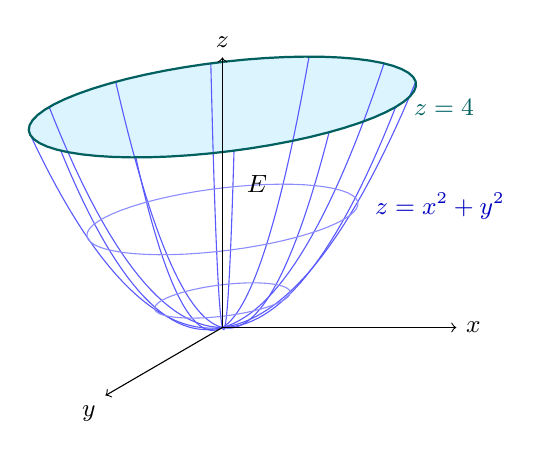
\begin{tikzpicture}[x={(1.1cm,0cm)},y={(-.55cm,-.32cm)},z={(0cm,.7cm)},every node/.style={font=\small}]
    \fill[cyan!14] plot[domain=0:360,samples=60] ({2*cos(\x)},{2*sin(\x)},4) -- cycle;
    \foreach \tt in {0,30,...,330} {
        \draw[blue!65] plot[domain=0:2,samples=30] ({\x*cos(\tt)},{\x*sin(\tt)},{\x*\x});
    }
    \foreach \rr in {.7,1.4} {
        \draw[blue!45] plot[domain=0:360,samples=60] ({\rr*cos(\x)},{\rr*sin(\x)},{\rr*\rr});
    }
    \draw[teal!75!black,thick] plot[domain=0:360,samples=60] ({2*cos(\x)},{2*sin(\x)},4);
    \draw[->] (0,0,0) -- (2.7,0,0) node[right] {$x$};
    \draw[->] (0,0,0) -- (0,2.7,0) node[below left] {$y$};
    \draw[->] (0,0,0) -- (0,0,4.9) node[above] {$z$};
    \node[right,teal!75!black] at (2.1,0,4) {$z=4$};
    \node[right,blue!75!black] at (1.65,0,2.2) {$z=x^2+y^2$};
    \node at (.4,0,2.6) {$E$};
\end{tikzpicture}
\end{center}
\endgroup
